\section{Web-Components}
\label{sec:3_Web_Components}

\todo[inline]{HTML Templates W3C Draft (18.März.2014) https://dvcs.w3.org/hg/webcomponents/raw-file/tip/spec/templates/index.html}
%http://www.w3.org/TR/html5/scripting-1.html#the-template-element

Um Web-Components besser verstehen zu können, wird in diesem Kapitel zu Beginn eine kurze Übersicht über die Geschichte von Web-Bibliotheken gezeigt.

\begin{description}
\item[2005] Veröffentlichung von Dojo Toolkit\footnote{Mehr Information zu Dojo Toolkit auf \href{http://dojotoolkit.org/}{http://dojotoolkit.org/}} mit der innovativen Idee von Widgets. Mit ein paar Zeilen Code konnten Entwickler komplexe Elemente, wie beispielsweise einen Graph oder eine Dialog-Box in ihrer Website hinzufügen.
\item[2006] jQuery\footnote{Mehr Information zu jQuery auf \href{http://jquery.com/}{http://jquery.com/}} stellt Entwicklern die Funktion zur Verfügung Plugins zu entwickeln, die später wiederverwendet werden können.
\item[2008] Veröffentlichung von jQuery UI\footnote{Mehr Information zu jQuery UI auf \href{http://jqueryui.com/}{http://jqueryui.com/}}, was vordefinierte Widgets und Effekte mit sich bringt.
\item[2009] Erstveröffentlichung von AngularJS\footnote{Mehr Information zu AngularJS auf \href{http://angularjs.org/}{http://angularjs.org/}}, ein Framework mit Direktiven.
\item[2011] Erstveröffentlichung von React\footnote{Mehr Information zu Facebook React auf \href{http://facebook.github.io/react/}{http://facebook.github.io/react/}}. Diese Bibliothek gibt den Entwicklern die Fähigkeit, das User Interface ihrer Website zu bauen, ohne dabei auf andere Frameworks, die auf der Seite benutzt werden, achten zu müssen
\item[2013] Veröffentlichung des Entwurfs von Web-Components, jedoch mit schlechter Browser Unterstützung
\end{description}

Mit der Veröffentlichung von Dojo Toolkit sagen Entwickler die Vorteile von wiederverwendbaren Modulen. Wenn man zurzeit Plugins auf einer Website erwähnt, denken die meisten Entwickler von jQuery Plugins, da sie beinahe überall Verwendung finden und ein großes Spektrum von Funktionen bieten. Mit den Veröffentlichungen von AngularJS und React wurde gezeigt, in welche Richtung sich Web-Anwendungen bewegen. Sie zeigen, dass es nicht nur um visuelle Elemente geht, sondern auch um Elemente, die eine komplexe Logik besitzen.




Ähnlich zu HTML5 ist Web-Components ein Sammelbegriff für mehrere Features:
\begin{description}
\item[Shadow DOM (ausführliche Erklärung siehe Kapitel \ref{sec:3_WC_Shadow_DOM} auf Seite \pageref{sec:3_WC_Shadow_DOM})] erlaubt es das DOM und CSS zu kapseln
\item[HTML Templates (ausführliche Erklärung siehe Kapitel \ref{sec:3_WC_Templates} auf Seite \pageref{sec:3_WC_Templates})] sind ein Weg, um den DOM zu klonen und somit den Klon wiederzuverwenden
\item[Custom Elements (ausführliche Erklärung siehe Kapitel \ref{sec:3_WC_Elements} auf Seite \pageref{sec:3_WC_Elements})] können einerseits neue Elemente definieren, oder bereits bestehende Elemente erweitern. Dies bedeutet, dass ein Entwickler beispielsweise den HTMl \lstinline|<input>|-Tag dahingehend erweitern kann, dass dieser nur das Format von Kreditkartennummern unterstützt. Ein Beispiel für die Definition eines neuen Elements wäre ein Element, dass sämtliche Felder, die für die Bezahlung mit einer Kreditkarte notwendig sind, bereitstellt.
\item[HTML Imports (ausführliche Erklärung siehe Kapitel \ref{sec:3_WC_Imports} auf Seite \pageref{sec:3_WC_Imports})] sind dazu da, um externe HTML-Dateien in die bestehende Website zu integrieren, ohne dabei den Code kopieren zu müssen. Sie können beispielsweise dazu verwendet werden, um Web-Components in eine Website zu integrieren.
\item[Decorators (ausführliche Erklärung siehe Kapitel \ref{sec:3_WC_Decorators} auf Seite \pageref{sec:3_WC_Decorators})] sind Elemente, die nach dem \glqq Decorator-pattern\grqq\ benannt sind. Durch dieses Pattern ist es möglich Elemente um zusätzliche Funktionalitäten zur Laufzeit erweitern zu können.
\end{description}

Obwohl \glqq Web-Components\grqq\ für viele Entwickler noch kein Begriff ist, wird es bereits vom Browser automatisch verwendet. Beispiele dafür sind der Datepicker oder das \lstinline|<video>|-Elemen. Abbildung \ref{fig:3_Datepicker_Visuals} auf Seite \pageref{fig:3_Datepicker_Visuals} zeigt die Datepicker-Komponente und Abbildung \ref{fig:3_Datepicker_Source} auf Seite \pageref{fig:3_Datepicker_Source} zeigt den dazugehörigen Source-Code. Dieser Code zeigt, dass sämtliche Kontrollbuttons des Datepickers vor dem Entwickler \glqq versteckt\grqq , also im Shadow DOM liegen.


\begin{figure}[h]
\centering
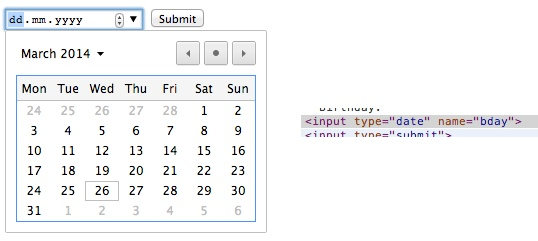
\includegraphics[height=5.0cm]{images/datepicker.jpg}
\caption[
Beispiel von Web-Components im Browser an Hand von dem Datepicker, Urldate: 04.2014 \newline
\small\texttt{https://s3.amazonaws.com/infinum.web.production/repository\_items/files/000/000/238/original/datepicker.jpg}
]{Beispiel von Web-Components im Browser an Hand von dem Datepicker}
\label{fig:3_Datepicker_Visuals}
\end{figure}

\begin{figure}[h]
\centering
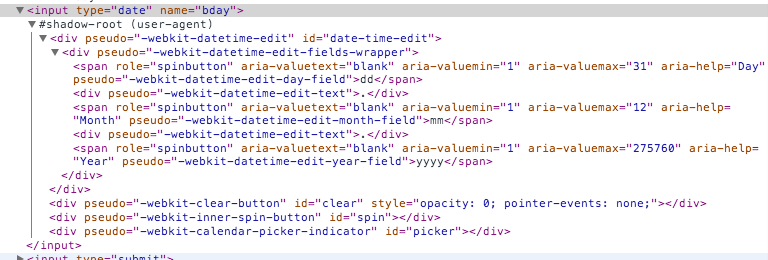
\includegraphics[height=5.0cm]{images/datepicker_shadow_dom.jpg}
\caption[
Beispiel von Web-Components im Browser an Hand von dem Datepicker, Urldate: 04.2014 \newline
\small\texttt{https://s3.amazonaws.com/infinum.web.production/repository\_items/files/000/000/236/original/datepicker\_shadow\_dom.jpg}
]{Beispiel von Web-Components im Browser an Hand von dem Datepicker}
\label{fig:3_Datepicker_Source}
\end{figure}

\textbf{Warum Web-Components?}\\
Javascript Widgets und Plugins sind fragmentiert, weil sie auf diversen unterschiedlichen Bibliotheken und Frameworks basieren, die möglicherweise nicht miteinander funktionieren. Web-Components versuchen einen gewissen Standard in Widgets und Plugins zu bringen. Das Problem der nicht miteinander funktionierenden Plugins versucht Web-Components mit Kapselung zu lösen. Durch die Lösung dieses Problems ist die Wiederverwendbarkeit von Komponenten garantiert, da es sämtliche Interferenzen zwischen Plugins löst. Web-Components können des Weiteren viel mehr als nur UI-Komponenten sein. Eine Bibliothek könnte bereits eine Komponente darstellen, die eine gewisse Funktionalität bereitstellt.

\textbf{Unterstützung von Web-Components}\\
Zur Zeit ist die Hauptproblem von Web-Components die mangelhafte Browserunterstützung. Kein einziger Browser unterstützt diesen Standard zu 100\%. Es gibt bereits mehrere Möglichkeiten beziehungsweise Polyfills\footnote{Ein Polyfill ist ein Browser-Fallback, um Funktionen, die in modernen Browsern verfügbar sind, auch in alten Browsern verfügbar zu machen.}, um dennoch Web-Components nutzen zu können. Beispiele hierfür sind:
\begin{itemize}
\item Polyfill-Webcomponents\footnote{Mehr Information zu Polyfill-Webcomponents unter \href{http://github.com/timoxley/polyfill-webcomponents}{http://github.com/timoxley/polyfill-webcomponents}}
\item Polymer-Project\footnote{Mehr Information zu Polymer unter \href{http://www.polymer-project.org/}{http://www.polymer-project.org/}}
\item X-tags\footnote{Mehr Information zu X-tags unter \href{http://x-tags.org/}{http://x-tags.org/}}
\end{itemize}
Obwohl es mehrere Polyfills bezüglich Web-Componnts gibt, ist es egal, auf welcher Basis man seine Web-Components programmiert, denn durch die Standardisierung ist die Interkompatibilität der einzelnen Komponenten gegeben. Diese Arbeit beschränkt sich hauptsächlich auf die Entwicklung von Web-Components mit Hilfe des Standards beziehungsweise der Polyfill-Bibliothek Polymer.\\
Durch die Benutzung von dem Polyfill Polymer funktionieren Web-Component in allen \glqq evergreen\grqq -Browsern\footnote{Ein \glqq Evergreen\grqq -Browser ist ein Web-Browser, der sich automatisch beim Start updatet.} und Internet-Explorer 10 und neuer. Des Weiteren funktionieren sie dadurch auf mobilen Endgeräten, wo iOS6+, Chrome Mobile, Firefox Mobile, oder Android 4.4 oder höher vorhanden ist. Auch mit Hilfe von Polyfill bieten sowohl der Internet-Explorer 9 und niedriger, als auch Android-Browser 4.3 oder niedriger keine Unterstützung für Web-Components. Dies bedeutet, dass Web-Components zur Zeit noch für die Verwendung im Web bereit sind, außer man hat als Zielgruppe ausschließlich eine Plattform, die unterstützt wird.

\textbf{Web-Components Alternativen}
Die folgenden Alternativen von Web-Components benutzen ähnliche Pattern um die gewünschte DOM-Abstrahierung zu erreichen.
\begin{description}
\item[React] benutzt seinen eigenen \glqq Virtual DOM\grqq und versucht in keinster Hinsicht Web-Components zu simulieren. Folglich ist die Browser-Unterstützung von React besser, als jene der Web-Components. Ab Internet-Explorer 8 werden sämtliche Browser vollständig unterstützt. Zur Zeit wird diese Technologie in Facebooks und Instagrams Kommentarsystemen eingesetzt.
\item[AngularJS] besitzt diverse Interferenzen zu Web-Components, jedoch versucht auch diese Technologie nicht Web-Components zu simulieren, um bessere Browser-Unterstützung zu bieten (Internet Explorer 8+). Die genaue Unterscheidung bezüglich AngularJS-Direktiven und Web-Components werden in Kapitel \ref{sec:3_Polymer} auf Seite \pageref{sec:3_Polymer} erklärt.
\end{description}



%\subsection{Relevanz von Web-Components hinsichtlich der Forschungsfrage}
%\label{sec:3_Relevanz}

\subsection{W3C Web-Components Standard}
\label{sec:3_W3C}

\subsubsection{Templates}
\label{sec:3_WC_Templates}

Das folgende Kapitel basiert ausschließlich auf der Spezifikation von Templates des W3C \citereset \autocite[siehe][]{Weinstein.2013} und auf dem Artikel \glqq HTML's new Template Tag\grqq\ \citereset \autocite[siehe][]{BidelmanTemplate.2013}.

Laut W3C sind Templates
\begin{quote}
\glqq
  a method for declaring inert DOM subtress in HTML and manipulating them to instantiate document fragments with identical contents.
\grqq
\end{quote}
Somit sind Templates eine Methode um inaktive DOM-Unterstruktur in HTML zu deklarieren und zu manipulieren, um so sämtliche identische Dokumentfragmente mit identischem Inhalt zu instanziieren.

In Web-Applikationen wird oft die gleiche Unterstruktur von Elementen wiederverwendet, mit dem passenden Inhalt gefüllt und zum Dokument hinzugefügt. Ein Beispiel in disem Kontext wäre eine Liste von Artikel, die mit mehreren \lstinline|<li>| -Tags in das Dokument eingefügt werden. Des Weiteren kann jeder \lstinline|<li>|-Tag weitere Elemente, wie beispielsweise einen Link, ein Bild, einen Paragraphen, etc., enthalten. Derzeit bot HTML keine native Möglichkeit an, eine solche Aufgabenstellung zu lösen.

Folgend wird eine Liste von Autos mit Hilfe eines Templates erstellt:
\begin{lstlisting}[language=HTML, caption={Web-Components Template-Standard}, label={lst:3_Templates}, escapeinside={@}{@}]
<template id="carTemplate">
  <li>
    <span class="carBrand"></span>
    <span class="carName"></span>
  </li>
</template>
\end{lstlisting}

Ein Template, wie das aus Code-Beispiel \ref{lst:3_Templates} auf Seite \pageref{lst:3_Templates}, kann sowohl im \lstinline|<head>|- als auch im \lstinline|<body>| definiert werden. Das Template, inklusive Subtree, ist inaktiv. Wenn sich ein \lstinline|<img>|-Tag mit einer validen Quelle in diesem Template befinden würde, würde der Browser dieses Bild nicht laden. Darüber hinaus ist es nicht möglich ein Element des Templates via JavaScript zu selektieren, wie in Code-Beispiel \ref{lst:3_Selector_Example} auf Seite \pageref{lst:3_Selector_Example} gezeigt wird.

\begin{lstlisting}[language=JavaScript, caption={Beispiel-Selektor eines Elements in einem Template, das nicht aktiven DOM ist}, label={lst:3_Selector_Example}]
  document.querySelectorAll('.carBrand').length; // length ist 0
\end{lstlisting}

\begin{figure}[h]
\centering
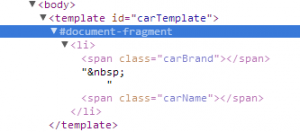
\includegraphics[height=3.0cm]{images/document_fragment.png}
\caption[
Visualisierung des DOM eines inaktiven Templates, Urldate: 04.2014
\newline
\small\texttt{\url{http://www.prevent-default.com/wp-content/uploads/2013/04/document-fragment-300x132.png}}
]{Visualisierung des DOM eines inaktiven Templates}
\label{fig:3_inactive_Template_DOM}
\end{figure}

In Abbildung \ref{fig:3_inactive_Template_DOM} auf Seite \pageref{fig:3_inactive_Template_DOM} wird gezeigt, dass das Template ein Dokument-Fragment ist. Dies bedeutet, dass es ein eigenständiges Dokument ist und unabhängig vom ursprünglichen Dokument existiert. Folglich bedeutet dies, dass sämtliche \lstinline|<script>, <form>, <img>, |-Tags etc. nicht verwendet werden können.

\begin{lstlisting}[language=JavaScript, caption={Verwendung des Templates \ref{lst:3_Templates} auf Seite \pageref{lst:3_Templates}}, label={lst:3_Templates_Verwendung}, escapeinside={@}{@}]
@\label{lst:3_Templates_Verwendung_1}@var template = document.getElementById('carTemplate');
template.content.querySelector(".carBrand").length; // length ist 1

@\label{lst:3_Templates_Verwendung_2}@var car = template.content.cloneNode(true);
car.querySelector(".carBrand").innerHTML = "Seat";
car.querySelector(".carName").innerHTML = "Ibiza";

@\label{lst:3_Templates_Verwendung_3}@document.getElementById("carList").appendChild(car);
\end{lstlisting}

Code-Beispiel \ref{lst:3_Templates_Verwendung} auf Seite \pageref{lst:3_Templates_Verwendung} basiert auf dem in Code-Beispiel \ref{lst:3_Templates} auf Seite \pageref{lst:3_Templates} definierten Template. Zu Beginn wird sich in Zeile \ref{lst:3_Templates_Verwendung_1} des Code-Beispiels \ref{lst:3_Templates_Verwendung} das bereits definierte Template in die Variable \lstinline|template| geholt. Daraufhin wird der gesamte Knoten in Zeile \ref{lst:3_Templates_Verwendung_2} mit Hilfe einer \lstinline|deep-copy| geklont und folglich mit Daten befüllt. Damit das mit Daten befüllte Listenelement auch sichtbar wird, wird es in Zeile \ref{lst:3_Templates_Verwendung_3} in das aktive DOM eingefügt.


\subsubsection{Decorators}
\label{sec:3_WC_Decorators}

\subsubsection{Custom Elements}
\label{sec:3_WC_Elements}

\subsubsection{Shadow DOM}
\label{sec:3_WC_Shadow_DOM}

\subsubsection{HTML Imports}
\label{sec:3_WC_Imports}

\subsubsection{Browser Unterstützung}
\label{sec:3_WC_Support}

\subsection{Google Polymer}
\label{sec:3_Polymer}
\todo[inline]{Unterscheidung zwischen predefined Elements, self-written custom Elements und Benutzung von Elementen}
\todo[inline]{Nesting von Elements bzw. Reuse beispielhaft zeigen}




\iffalse
%STACKOVERFLOW POLYMER
In general, Polymer is a framework that aims to use (and show how to use) Web Components. It's foundation is Custom Elements (e.g. everything you build is a web component) and it evolves as the web evolves. To that end, we only support the latest version of the modern browsers.

I'll use this image to describe Polymer's entire architecture stack:
%polymers architecture http://i.stack.imgur.com/Ksn6s.png

RED layer: We get tomorrow's web through a set of polyfills. Keep in mind, those libraries go away over time as browsers adopt the new APIs.

YELLOW layer: Sprinkle in some sugar with polymer.js. This layer is our opinion on how to use the spec'd APIs, together. It also adds things like data-binding, syntatic sugar, change watchers, published properties...We think these things are helpful for building web component-based apps.

GREEN: The comprehensive set of UI components (green layer) is still in progress. These will be web components that use all of the red + yellow layers.

%STACKOVERFLOW END

How is Polymer different from Angular JS Directive? (Fundamentally and technologically)

Polymer (and more correctly, Shadow DOM) create the ability to not only compose bits of HTML, but to encapsulate them as well. This is a fundamentally new capability and one that can be used with any other templating system or framework to enhance their power.

In terms of templating/interpolation, Polymer uses MDV which does bi-directional data binding in a similar way to Angular for older browsers, but in newer runtimes can take advantage of Mutation Observers and eventually Object.observe() to help speed up change detection and propagation.
\fi



Ein Beispiel für ein vordefiniertes Element der Google-Polymer Bibliothek wäre das \lstinline|<polymer-ajax>|-Element. Es erscheint in erster Linie als nicht sehr nützlich, jedoch versucht es, einen Standard für Entwickler bereitzustellen, um Ajax-requests zu erstellen beziehungsweise abzuwickeln. Dieses Element ist ähnlich zu folgender Funktion: \lstinline|\$.ajax()|\footnote{Mehr Information zur jQuery.ajax-Funktion unter \href{http://api.jquery.com/jQuery.ajax/}{http://api.jquery.com/jQuery.ajax/}}. Der Unterschied zwischen den beiden Möglichkeiten, einen Ajax-Request abzuwickeln, ist, dass die \lstinline|\$.ajax()|-Methode Abhängigkeiten besitzt, wohingegen die \lstinline|<polymer-ajax>|-Methode vollkommen unabhängig ist.

\subsection{Konklusion}
\label{sec:3_Konklusion}



